\subsection{Casi d'uso}
In questa sezione sono riportati i casi d'uso relativi alla prima versione dell'applicazione, sia in forma testuale che come diagramma UML.\bigskip 

Nella descrizione testuale di tutti i casi d'uso eccetto "Creazione configuratore" e "Accesso configuratore" è lasciato sottinteso il fatto che l'utente debba aver effettuato l'accesso al proprio profilo prima di poter proseguire con l'interazione descritta dal caso d'uso considerato: la scelta relativa all'azione da effettuare e di conseguenza del caso d'uso a cui far riferimento avviene infatti tramite un menu presentato all'utente solo dopo aver effettuato l'accesso, pertanto non sarebbe possibile richiedere di effettuare alcuna operazione che non sia la creazione di un nuovo profilo Configuratore o l'accesso a un profilo già esistente prima che venga presentato suddetto menu.\bigskip

Nella Tabella \ref{tab:Use Case 1.1} è riportato il caso d'uso testuale relativo all'accesso dell'utente configuratore al proprio profilo: l'utente interagisce con l'applicazione inserendo il proprio username e password; in questo caso d'uso, pertanto, è incluso il caso d'uso ``Creazione configuratore" che viene invocato nella situazione in cui non esista ancora alcun utente registrato.\bigskip

Nella Tabella \ref{tab:Use Case 1.2} è riportato il caso d'uso testuale relativo alla creazione di un nuovo profilo configuratore: l'utente riceve la comunicazione delle proprie credenziali temporanee, accede al proprio profilo e modifica le proprie credenziali a piacere (rispettando il vincolo relativo all'univocità dello username).\bigskip

Nella Tabella \ref{tab:Use Case 1.3} è riportato il caso d'uso testuale relativo alla creazione di una nuova gerarchia da parte dell'utente configuratore: l'utente, dopo aver effettuato l'accesso, interagisce con l'applicazione chiedendo di aggiungere nuove categorie oppure salvare la configurazione esistente; in questo caso d'uso, pertanto, sono inclusi i casi d'uso ``Aggiunta categoria" e ``Salvataggio dati", a cui si demandano i compiti relativi.\bigskip

Nella Tabella \ref{tab:Use Case 1.4} è riportato il caso d'uso testuale relativo alla Visualizzazione di tutte le gerarchie presenti all'interno dell'applicazione da parte dell'utente configuratore.\bigskip

Nella Tabella \ref{tab:Use Case 1.5} è riportato il caso d'uso testuale relativo all'aggiunta di una categoria a una gerarchia; si tratta di un caso d'uso incluso in quello relativo alla creazione di una gerarchia.\bigskip

Nella Tabella \ref{tab:Use Case 1.6} è riportato il caso d'uso testuale relativo al salvataggio dei dati introdotti nell'applicazione dall'utente configuratore.\bigskip

In Figura \ref{fig:Use Case 1} è riportato il diagramma UML dei casi d'uso relativo alla prima versione dell'applicazione. Dall'immagine possiamo ricavare facilmente che i casi d'uso \textit{sea-level}, ossia quelli corrispondenti agli obiettivi per cui l'utente interagisce con l'applicazione, sono:
\begin{itemize}
    \item Creazione di un nuovo profilo configuratore 
    \item Accesso a un profilo configuratore già esistente
    \item Creazione di una gerarchia di categorie
    \item Visualizzazione di tutte le gerarchie di categorie presenti nell'applicazione
    \item Salvataggio dei dati dell'applicazione
\end{itemize}
Alcuni di questi casi d'uso \textit{sea-level} sono interpretabili come casi d'uso \textit{fish-level} laddove vengano inclusi da un altro caso d'uso al fine del raggiungimento dell'obiettivo per cui l'utente interagisce con l'applicazione.

L'unico caso d'uso che ha natura esclusivamente \textit{fish-level} è quello relativo all'aggiunta di una nuova categoria a una gerarchia, in quanto esso è incluso nel caso d'uso "Creazione gerarchia". Inoltre, i casi d'uso "Creazione configuratore" e "Salvataggio dati" sono inclusi in altri casi d'uso \textit{sea-level}, pertanto possono essere visti anche come casi d'uso \textit{fish-level} oltre che \textit{sea-level}.

\begin{figure}[hb]
\centering
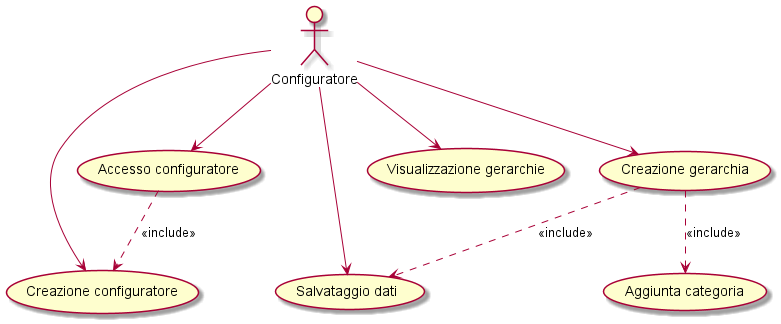
\includegraphics[width=0.9\textwidth]{imagesV1/Use case diagram-Version 1.0.png}
\caption{\label{fig:Use Case 1}Diagramma UML dei casi d'uso - Versione 1}
\end{figure}\bigskip